\section{Firewall Konfiguration}

\newcommand{\lstfwa}[2]{
\lstinputlisting[
    firstline=#1,
    lastline=#2,
    firstnumber=#1
]{code/firewall-external.sh}
}

\newcommand{\lstfwb}[2]{
\lstinputlisting[
    firstline=#1,
    lastline=#2,
    firstnumber=#1
]{code/firewall-internal.sh}
}

Die Paketprüfung mit {\tt iptables} ist dreistufig aufgebaut.
Hierarchisch von oben nach unten angeordnet gibt es die Tabellen, die Chains
(Ketten) und die eigentlichen Filterregeln\footnote{
\url{http://wiki.ubuntuusers.de/iptables2}
}.
Die im Rahmen des Labors verwendeten Tabellen sind einerseits die {\tt filter}
Tabelle, welche reine Filterregeln enthält, und die {\tt nat} Tabelle, welche
für Network Address Translations und Verfahren wie Port Forwarding eingesetzt
wird.
Innerhalb jeder Tabelle existieren verschiedene Chains, welche spezifizieren,
wann ein Paket geprüft wird.
Folgende Chains existieren in den Linux {\tt iptables}:

\begin{itemize}
\item {\tt INPUT} --- betrifft Pakete, welche an einen lokalen Prozess gehen
      sollen.
\item {\tt OUTPUT} --- betrifft Pakete, welche von einem lokalen Prozess stammen.
\item {\tt FORWARD} --- betrifft Pakete, welche geroutet werden.
\item {\tt PREROUTING} --- wird auf Pakete angewendet, bevor diese geroutet
      werden (Element der {\tt nat} Tabelle).
\item {\tt POSTROUTING} --- wird auf Pakete angewendet, nachdem diese geroutet
      wurden (Element der {\tt nat} Tabelle).
\end{itemize}

\noindent Die eigentlichen Regeln werden in einer Tabelle und Chain definiert,
trifft eine Regel auf ein Paket zu, wird die in der Regel angegebene Aktion
durchgeführt.
Wenn keine Regel zutrifft, wird die allgemein gültige Policy angewendet.

\begin{figure}[h!]
  \centering
    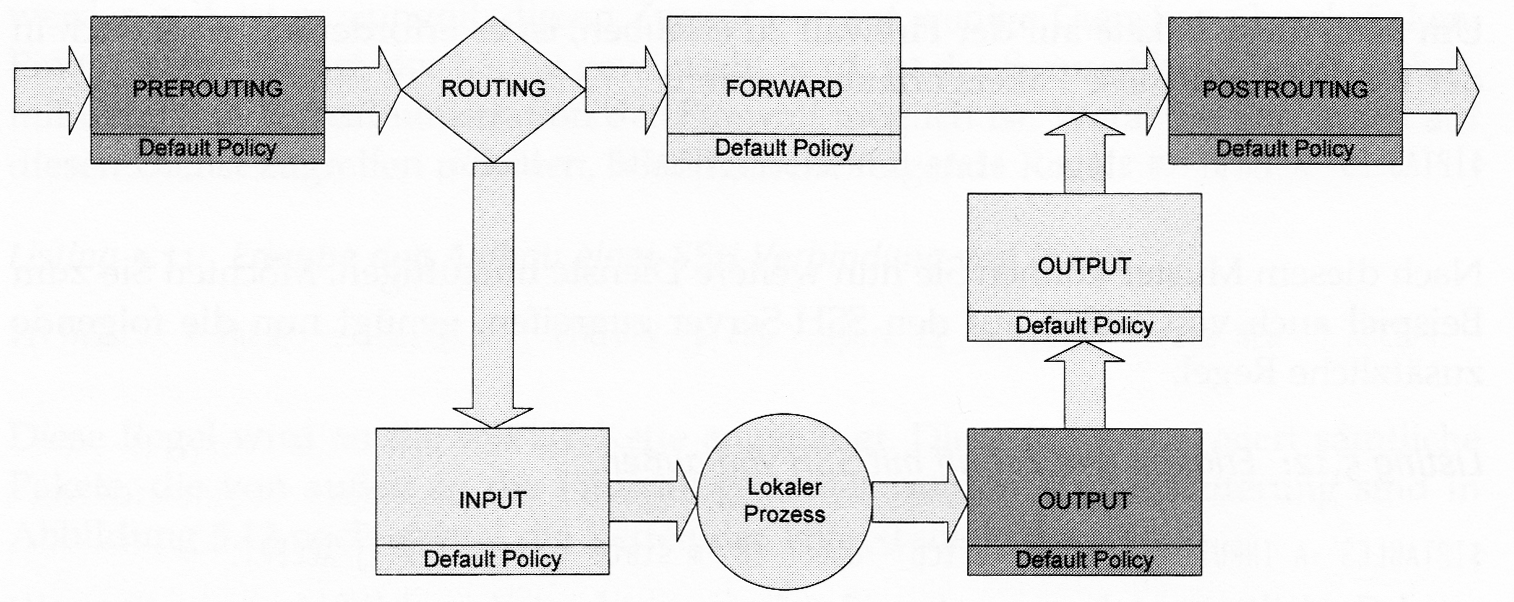
\includegraphics[width=0.99\textwidth]{figures/iptables-filter-nat.png}
  \caption{Filter- und NAT-Tabelle von {\tt iptables}. Aus \cite{iptables} Abb. 5.13.}
  \label{fig.iptables-filter-nat}
\end{figure}

\noindent Als grundsätzliche Konfiguration beider Firewalls wird die Policy für
eingehende, ausgehende und weiterzuleitende Pakete auf {\tt DROP} gesetzt.
Dies wird mit den {\tt iptables} Befehlen aus Listing \ref{lst:policy}
realisiert.

\lstinputlisting[
    firstline=39,
    lastline=41,
    label=lst:policy,
    caption={Default-Policy der Firewalls.}
]{code/firewall-external.sh}

\noindent Da die Firewall Rechner als Router zwischen den jeweiligen Netzen
fungieren, muss grundsätzlich das Forwarding von Paketen aktiviert werden.
Für IPv4-Pakete kann dafür der folgende Befehl genutzt werden:

\begin{verbatim}
echo "1" > /proc/sys/net/ipv4/ip_forward
\end{verbatim}

\noindent Um die Kommunikation lokaler Dienste nicht zu stören, werden ein-
und ausgehende Pakete an die Loopback-Adresse ({\tt 127.0.0.1}) nicht von der
Firewall blockiert.
Für die weiterzuleitenden Pakete wird Connection Tracking
(siehe Kapitel \ref{sec.fw-tec}) verwendet.
Damit in den eigentlichen Regeln nur noch Pakete mit Status {\tt NEW} erlaubt
werden müssen, werden Pakete mit Status {\tt ESTABLISHED} oder {\tt RELATED}
grundsätzlich erlaubt.
{\tt INVALID} Pakete dagegeben werden vor allen anderen Regeln verworfen.

\lstinputlisting[
    firstline=49,
    lastline=61,
    label=lst:established_related_invalid,
    caption={Regeln für ESTABLISHED, RELATED und INVALID Pakete.}
]{code/firewall-external.sh}


\subsection{\fwa}\label{sec.konfig.fwa}

Die Konfigurationsdatei für {\tt fw1} aus Listing \ref{lst:external}
befindet sich in\\
{\tt /etc/init.d/firewall-external.sh}.
Das Skript wird mit dem Befehl\\
{\tt chmod u+x firewall-external.sh}
ausführbar gemacht und mit\\
{\tt insserv firewall-external.sh}
wird das Skript auch beim Aufstarten der Maschine automatisch ausgeführt,
und damit die Firewall aktiviert.

\paragraph{§ 1 Zugriff auf das Internet}

Damit {\tt fw1} die Pakete zum LAN weiterleiten kann, wird mit dem folgenden
Befehl eine Route zum LAN in die Routingtabelle eingetragen.
Dabei wird {\tt fw2} als Gateway verwendet.
\lstfwa{47}{47}

\noindent Damit die zum Extranet gehenden Pakete die öffentliche IP-Adresse
von Firma A enthalten, werden die Paketheader in der POSTROUTING Kette der
{\tt nat} Tabelle umgeschrieben.
Es werden die IP-Adressen von {\tt srv1} und die des gesamten LANs
umgeschrieben.
Mit dem FORWARD Befehl wird die Weiterleitung aller Verbindungen,
welche aus dem LAN ins Extranet aufgebaut werden, erlaubt.

\lstfwa{74}{79}

\noindent Allgemein sieht der FORWARD Befehl folgendermaßen aus:

\begin{verbatim}
iptables -A FORWARD ... -m conntrack --ctstate NEW -j ACCEPT
\end{verbatim}

\noindent Statt {\tt ...} können folgende Parameter eingesetzt werden,
mit denen sich die Verbindung spezifizieren lässt.

\begin{itemize}
  \item {\tt -i} gibt das Netzwerkinterface an, wo das Paket empfangen wird
  \item {\tt -o} gitt das Netzwerkinterface an, über das das Paket gesendet werden soll
  \item {\tt -s} gibt das Quellnetzwerk bzw. die Quell-IP-Adresse an
  \item {\tt -d} gibt das Zielnetzwerk bzw. die Ziel-IP-Adresse an
  \item {\tt -p / --dport} spezifiziert das Protokoll. Möglich sind dabei tcp, udp und icmp. Mit {\tt --dport} kann ein Zielport angegeben werden.
\end{itemize}

\paragraph{§ 2 Mail- und Webserver}

Da mehrere Ports zu {\tt srv1} weitergeleitet werden müssen, wurde folgende
Shell-Funktion definiert.
Die Ziel-IP-Adresse wird mit DNAT in der PREROUTING Kette modifiziert,
die neue Ziel-IP-Adresse wird mit {\tt --to} am Ende des Befehls angegeben.
Zusätzlich wird die Weiterleitung der so modifizierten Pakete erlaubt.

\lstfwa{23}{28}

\noindent Dies ist der Shell-Funktionsaufruf um die jeweilige Portfreigabe
durchzuführen:

\lstfwa{67}{72}

\paragraph{§ 3 VPN}

Für VPN wird ebenfalls Port-Forwarding verwendet, dieses Mal werden
die Pakete jedoch an {\tt fw2} weitergeleitet.

\lstfwa{85}{91}

\paragraph{§ 4 DNS}

Damit der interne DNS-Server auf {\tt srv1} DNS-Anfragen an {\tt net1}
durch\-führen kann, wird diese Regel verwendet:

\lstfwa{82}{83}

\paragraph{§ 5 Sonstiges}

Zu Testzwecken wurden zudem eingehende Echo Requests (ping) erlaubt.

\lstfwa{64}{64}

\noindent Alle Pakete, die nicht auf eine der bisherigen Regeln zutreffen,
werden in einer Logdatei aufgezeichnet und verworfen.

\lstfwa{93}{99}

\subsection{\fwb}

Die Konfigurationsdatei für {\tt fw2} aus Listing \ref{lst:internal}
befindet sich in\\
{\tt /etc/init.d/firewall-internal.sh} und wird mit den Befehlen
aus Kapitel \ref{sec.konfig.fwa} ausführbar gemacht.

\paragraph{§ 1 Zugriff auf das Internet}

{\tt fw2} verwendet {\tt fw1} als Gateway zum Extranet.

\lstfwb{48}{48}

\noindent Alle Verbindungsaufbauten aus dem internen Netzwerk ins Extranet
werden erlaubt.

\lstfwb{65}{65}


\paragraph{§ 2 Mail- und Webserver}

Definition der Shell-Funktion:

\lstfwb{24}{29}

\noindent Die folgenden TCP Ports werden weitergeleitet:

\lstfwb{75}{80}

\paragraph{§ 3 VPN}

Definition der beiden VPN-Netzwerkadapter. Hier wurde nur eine Dummy Config
verwendet, da kein VPN-Dienst konfiguriert ist.

\lstfwb{21}{22}

\noindent Es müssen die eingehenden Pakete an die UDP Ports 1194 und 1195
erlaubt werden.
Beidseitiger VPN-Verkehr wird zwischen dem jeweiligen VPN-Netzwerkadapter
und dem internen Netzwerk gestattet.

\lstfwb{84}{92}

\paragraph{§ 4 DNS}

Die Rechner aus dem internen Netzwerk erhalten Zugriff auf den DNS-Server
von {\tt srv1}.

\lstfwb{81}{82}

\paragraph{§ 5 Sonstiges}

Es werden die gleichen Logging-Regeln wie für {\tt fw1} verwendet.
Für die Rechner aus dem internen Netzwerk wird
ein Echo Request (ping) auf {\tt fw2}, {\tt fw1} und {\tt srv1} erlaubt.

\lstfwb{67}{72}



\newpage
\section{Tests}\label{sec.tests}

\paragraph{§ 1 Zugriff auf das Internet, § 4 DNS}

Mit dem {\tt pc01.firma-a.f223} wird via Webbrowser die Internetseite
von {\tt net1.internet.f223} aufgerufen.
Damit kann gezeigt werden:
\begin{itemize}
  \item DNS-Auflösung aus § 4 der Anforderungen des Hostnames funktioniert.
  \item Ein unbeschränkter Zugriff aus dem internen Netzwerk ins Internet
        ist möglich.
  \item Das Masquerading funktioniert, da sonst keine Rückantwort möglich wäre,
        weil das interne Netzwerk aus Sicht des Internets hinter der
        öffentlichen IP-Adresse versteckt ist.
\end{itemize}

\noindent Grundsätzlich wurden alle Verbindungen mittels {\tt iptstate} analysiert.
Für den oben angegebenen Testfall zeigen die Abbildungen
\ref{fig.iptstate-extern} und \ref{fig.iptstate-intern} die existierenden
Verbindungen an.

\begin{figure}[h!]
  \centering
    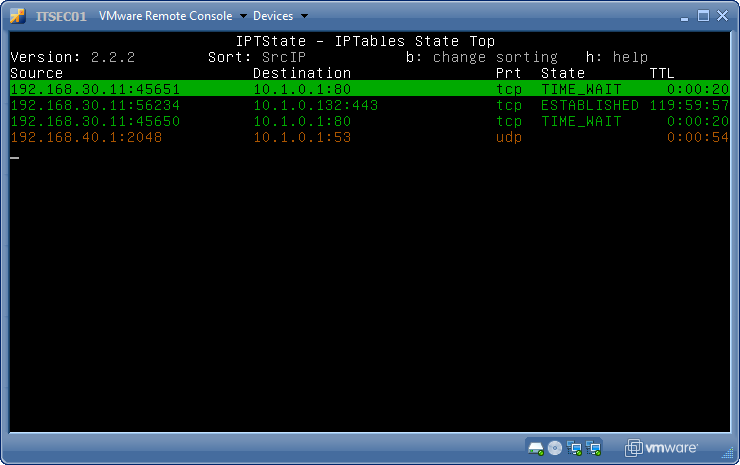
\includegraphics[width=0.9\textwidth]{figures/iptstate-extern.png}
  \caption{{\tt iptstate} der externen Firewall.}
  \label{fig.iptstate-extern}
\end{figure}

\begin{figure}[h!]
  \centering
    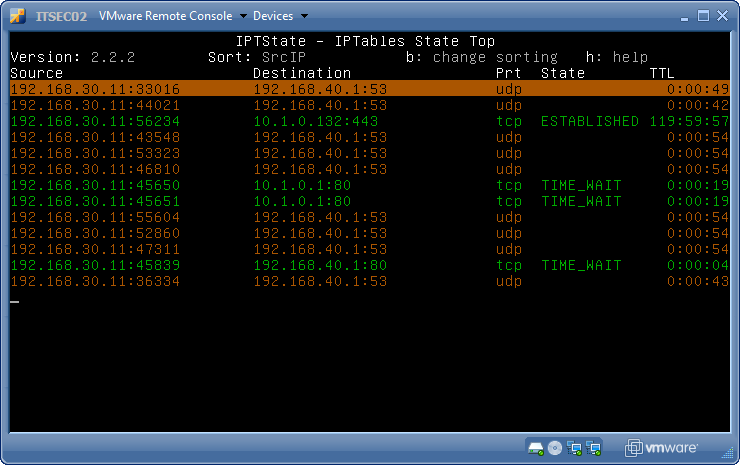
\includegraphics[width=0.9\textwidth]{figures/iptstate-intern.png}
  \caption{{\tt iptstate} der internen Firewall.}
  \label{fig.iptstate-intern}
\end{figure}


\paragraph{§ 2 Mail- und Webserver}

{\tt pc01.firma-a.f223} aus dem internen Netzwerk hat auf
den Webserver von {\tt srv1.firma-a.f223} Zugriff.

Der externe Zugriff auf Mail- und Webserver wird mit {\tt lap01.internet.f223}
getestet.
Dies zeigt, dass das Port-Forwarding von {\tt fw1} zu {\tt srv1}
wie gewünscht funktioniert.

\paragraph{§ 3 VPN}
konnte nicht getestet werden, da auf dem neu aufgesetzten Firewall-Rechner
{\tt fw2} kein VPN-Server konfiguriert ist.


\subsection{Netzwerkkonfiguration von {\tt srv1}}

Damit beim Zugriff von einem Rechner aus dem LAN auf den Server
{\tt srv1} der \emph{Firma A} die Pakete direkt zurückgesendet werden und nicht
erst beim Default-Gateway {\tt fw1} landen, wurde auf dem
Server eine Route zum LAN mit {\tt fw2} als Gateway definiert.
Dafür wurde folgende Zeile zur Datei {\tt /etc/network/interfaces} hinzugefügt:
\begin{verbatim}
up route add -net 192.168.30.0/24 gw 192.168.40.240
\end{verbatim}


\newpage
\section{Zusammenfassung}

In diesem Praktikumsversuch konnten wir lernen, wie man das Firewall-Konzept
einer multiplen DMZ umsetzt. Dabei wurde die im Linux-Kernel vorhandene
{\tt iptables} Technologie verwendet, wobei als Linux-Distribution Debian 6.0
mit dem Codenamen „Squeeze“ zum Einsatz kam.
\\ \\
\noindent Das Labor ist als virtuelles Labor vorgesehen, d.h. sämtliche Rechner liegen
als virtuelle Maschinen vor, was ein einfacheres Testen und Debuggen ermöglicht.
Somit kann jede Gruppe autonom an ihrer Aufgabenstellung arbeiten.
\\ \\
\noindent Das Firewall-Konzept muss folgenden Anforderungen genügen:

\begin{itemize}
  \item Vom internen Netzwerk Zugriff auf das Internet.
  \item Bestimmte Dienste in der DMZ sollen vom Internet aus erreichbar sein.
  \item VPN-Zugriffe auf das interne Netzwerk sollen möglich sein.
\end{itemize}

\noindent Abschließend möchten wir uns bei Frau Dr. Düsterhöft für die
kompetente und tatkräftige Laborbetreuung bedanken.
